\chapter{azLinux}

Чтобы разобраться как можно собрать встраивамый \linux, в этом разделе описан
набор \make-файлов и файлов конфигурации для сборки минимального \emlinux.
Это обрезанный форк проекта \href{https://github.com/user/cross}{Cross
Linux}, подробнее описанного в разделе \ref{cross}. Ограничено количество
поддерживаемого железа, упрощены конфигурационные файлы, минимизировано
количество библиотек и программных пакетов.

\bigskip 

Изначально идея создания этой системы появилась из желания заменить тухлую
связку x86/DOS/Tur\-bo\-Pas\-cal на что-то

\begin{itemize}
  \item \emph{более переносимое}: на
 энергоэффективное ARM/MIPS-железо, в т.ч. (типа)отечественного производства,
\item \emph{стабильное}: с полноценной многозадачностью,
защитой памяти и данных, и
\item \emph{позволяющее использовать максимум возможностей аппаратуры}: большая
\ram, ECC, gcc-оп\-ти\-ми\-зи\-ро\-ван\-ный 32/64-битный код, USB, CAN, Ethernet,
WiFi, разнообразные носители данных, аппаратный watchdog.

\item Также большой интерес представляют \emph{десятки готовые библиотек} сжатия
и кодирования данных, численных методов, ЦОС, и обработки изображений, а также

\item множество \emph{готовых программ, доступных в исходных кодах}\note{для
использования как есть, изучения принципов работы и модификации под
собственные нужды}\ для выполнения различных полезных функций: сетевые серверы,
символьная математика, обработка данных,\ldots

\item Еще одна ключевая фича\ --- \emph{способность}\ \linux\ полностью
\emph{загружаться в \ram\ с \textbf{любых} носителей, в т.ч. заблокированных на
запись}. Это важно для случаев, когда возможны внезапные выключения питания:
вся система работает в \ram-диске, а корректность записи данных на изменяемые
носители можно гибко контролировать программно. При запуске после аварийного
выключения никаких проверок файловых систем не требуется, ОС стартует сразу, а
проверку/починку разделов данных возможно выполнять в фоновом режиме.

\item \emph{Время запуска системы}\ --- на x86 удалось экспериментально получить
время запуска \emph{0.2\,сек от загрузки ядра до начала выполнения
пользователького кода}.
Используя модульное ядро, возможно выполнить критический к времени запуска
пользовательский код до инициализации USB, сети, внешних носителей данных и
тяжелых сервисов.

\end{itemize}

\paragraph{Почему не BuildRoot}

Эта система сборки создавалась как \emph{максимально облегченный пакет
для решения узких задач}, и для освоения технологии кросс-компиляции.
Предполагается что функциональное наполнение не будет развиваться шире набора:

\begin{itemize}
  \item ядро (реального времени)
  \item libc
  \item урезанная командная оболочка (busybox)
  \item несколько прикладных библиотек поддержки (сжатие, кодирование, базовая
  графика)
  \item пользовательский узкоспециализированный код на Си/\cpp
\end{itemize}

Расширять функционал, добавляя libQt, X Window, Apache, MySQL,\ldots, Gnome/KDE
и т.д. не планируется в принципе\ --- \emph{это система для решения узких
прикладных задач}\ на аппаратуре с минимальными ресурсами\note{особенно
интересны процессорные модули в DIMM форм-факторе, только CPU, RAM,
NAND и GPIO гребенка}. \emph{Интерактивная работа}\ с пользователем также
\emph{не предполагается}, доступна только командная консоль\note{ее можно
считать сервисным режимом}, и очень ограниченные графические и мультимедийные
возможности. Если ваши хотелки выходят за этот функционал, рекомендую сразу
уходить на использование ширко известной системы кросс-сборки \linux-систем под
названием \file{BuildRoot}\ref{buildroot}.

\section{Требования к системе сборки (\file{BUILD}-хост)}

Требования жесткие\ --- 2х-ядерный процессор, 2+\,Гб \ram, для 4+\, Гб \ram\
нужен 64х-битный дистрибутив \linux\ (рекомедую Debian), и естественно никаких
виртуалок.
Возможна установка системы на флешку, в этом случае требования к \ram\ еще более
ужесточаются\ --- потребуется каталоги с временными файлами смонтировать как
\file{tmpfs}:

\lst{добавить в \file{/etc/fstab}}{}{azlin/doc/fstab.txt}

Можно попытаться сделать \term{билд-сервер}\ и на худшем железе, но будьте
готовы к тормозам или внезапному окончанию памяти\ --- ресурсоемка сборка
тяжелых библиотек типа \prog{libQt}\ или крупных пакетов типа \prog{gcc}.

Вы можете попробовать поставить \linux\ на виртуалку, на флешку, и на жесткий
диск (если найдете место) и оценить возможности этих вариантов на сборке пакета
\prog{gcc0}. При сборке с флешки на ноутбуке с 2\,Гб \ram\ мне для сборки
\prog{gcc0}\ пришлось временно размонтировать \file{cross/src}, сделать
\file{./mk.rc \&\& make gcc ramclean}, а потом примонтировать \file{tmpfs}\
опять на \file{src}.

Сборка под MinGW/Cygwin совершенно неживая. Если совсем никак без винды\ ---
используйте виртуалки, и будьте готовы ждать.

\section{Понятие \term{пакет}}

Прежде чем продолжить, введем понятие \term{пакет}. В az\linux\ \term{пакетом}\
называется одна или несколько частей скриптов сборки, обозначаемых именем. В
чем-то это похоже на бинарные пакеты обычных дистрибутивов \linux\ --- чтобы
добавить в систему какой-то функционал, мы устанавливаем \term{бинарный пакет}.
Но есть и отличие: пакет дистрибутива это реальный архивный файл, содержащий в
себе файлы программ, данных; в az\linux\ пакет\ --- виртуальная штука с именем.

Просматривая файлы в каталоге \file{mk/}, легко найти имена пакетов по шаблону:

\begin{verbatim}
.PHONY: somename
somename: [зависимые файлы]
    [команда1]
    ...
\end{verbatim}

Если вы запустите команду:

\begin{verbatim}
cd ~/az ; ./mk.rc && make somename
\end{verbatim}

запустится \term{сборка пакета}\ \pack{somename}.

Но не нужно забывать, что кроме этой секции в \file{.mk}, существуют зависимости
между файлами, при работе команд сборки динамически создаются и изменяются
файлы, иногда что-то скачивается из \internet а\ --- все эти процессы тоже
входят в пакет.

\bigskip
Часть пакетов не связана со сборкой программ, а выполняют служебные функции,
поэтому для них правильнее будет фраза \term{запуск пакета}.

\bigskip
Все действия выполняются с помощью команды \prog{make}. Обратите особое
внимание на то, что \file{Makefile}\ собирается скриптом \prog{mk.rc}\ из частей
в каталоге \file{mk/}, поэтому \emph{если вы что-то меняете в скриптах, не
забудьте сначала запустить \prog{./mk.rc}}.

\lstx{mk.rc}{}{../azlin/mk.rc}{rc}\index{azLinux!скрипт!mk.rc}

\section{Загрузка}

При необходимости вносить правки\note{что естественно\ --- вам потребуется
добавлять свои пакеты и поддержку железа}\ работайте с вашим
собственным форком на GitHub.

Получите клон пакета из репозитория:

\begin{verbatim}
cd ~ ; git clone --depth=1 -o gh https://github.com/user/azlin az
\end{verbatim}

При необходимости обновитесь:

\begin{verbatim}
cd ~/az ; git pull
\end{verbatim}

\section{Общий порядок сборки}

Каждый пакет собирается командой:

\begin{verbatim}
./mk.rc && make [HW=rpi] [APP=clock] <package>
\end{verbatim}

\begin{enumerate}
  \item \prog{dirs} создание дерева каталогов \ref{azdirs} 
  \item \prog{gz} закачка архивов исходников \ref{azgz} 
  \item \prog{tc} сборка кросс-компилятора \ref{aztc}
  \begin{enumerate}
    \item \prog{binutils} ассемблер, линкер и утилиты \ref{azbinutils}
    \item \prog{cclibs} библиотеки для сборки \prog{gcc} \ref{azcclibs}
    \item \prog{gcc0} сборка минимального кросс-компилятора Си \ref{azgcc0}
  \end{enumerate}
  \item \prog{core} сборка основной системы \ref{azcore}
  \begin{enumerate}
    \item \prog{kernel} ядро \linux\ \ref{azkernel}
    \item \prog{libc} библиотека \prog{uClibc} \ref{azlibc}
    \item \prog{bb} набор утилит \prog{busybox} \ref{azbb}
    \item \prog{gcc} пересборка полного \prog{gcc} \ref{azgcc}
  \end{enumerate}
  \item \prog{libs} сборка библиотек \file{\$\{LIBS\}} \ref{azlibs}
  \item \prog{apps} сборка прикладных пакетов \file{\$\{APPS\}} \ref{azapps}
  \item \prog{user} сборка пользовательского кода \ref{azuser}
  \item \prog{root} формирование корневой файловой системы \ref{azroot}
  \item \prog{boot} сборка загрузчика \ref{azboot}
  \item \prog{emu} запуск собранной системы в эмуляторе \ref{azemu}
  \item \prog{netboot} сетевая загрузка \ref{aznetboot}
  \item \prog{firmware} прошивка на устройство \ref{azfirmware}
\end{enumerate}

\section{Фиксация переменных}

Если вам требуется собрать систему со значениями переменных, отличающихся от
тех, которые прописаны в make-файлах, при запуске \emph{всех}\ пакетов нужно
указывать трюбуемые значения в командной строке. Это позволить легко выбрать
нужный вам вариант сборки.

\begin{verbatim}
./mk.rc && make HW=rpi APP=clock distclean dirs tc core libs apps boot root
\end{verbatim}

При таком указании все переназначения для этих переменных игнорируются, поэтому
возможны некоторые сложности с указанием например опций оптимизации.

\section{dirs: Создание дерева каталогов}

После загрузки или обновления запустите пакет \prog{dirs}:

\begin{verbatim}
$ ./mk.rc && make dirs
mkdir -p /home/user/Azbuka/azlin/gz /home/user/Azbuka/azlin/src
/home/user/Azbuka/azlin/tmp /home/user/Azbuka/azlin/x86_64-linux-gnu
/home/user/Azbuka/azlin/qemu386-clock /home/user/Azbuka/azlin/qemu386-clock/boot
\end{verbatim}
\begin{verbatim}
$ ls -la
итого 72
drwxr-xr-x 2 user user  4096 Дек  8 11:43 app
drwxr-xr-x 2 user user  4096 Дек  8 11:43 arch
-rw-r--r-- 1 user user 17699 Дек  8 13:25 azlin.tex
drwxr-xr-x 2 user user  4096 Дек  8 11:43 cpu
drwxr-xr-x 2 user user  4096 Дек  8 13:26 gz
drwxr-xr-x 2 user user  4096 Дек  8 11:43 hw
-rw-r--r-- 1 user user  2087 Дек  8 13:26 Makefile
drwxr-xr-x 2 user user  4096 Дек  8 11:43 mk
-rwxr-xr-x 1 user user   121 Дек  8 11:43 mk.rc
drwxr-xr-x 3 user user  4096 Дек  8 13:26 qemu386-clock
-rw-r--r-- 1 user user   147 Дек  8 11:43 README.md
drwxr-xr-x 2 user user  4096 Дек  8 13:26 src
drwxr-xr-x 2 user user  4096 Дек  8 13:26 tmp
drwxr-xr-x 2 user user  4096 Дек  8 13:26 x86_64-linux-gnu
\end{verbatim}

Пакет \prog{dirs}\ прописан в файле

\lstx{mk/dirs.mk}{}{../azlin/doc/dirs.mk}{mk}\index{azLinux!пакет!dirs}

Встроенная переменная \file{PWD}\ содержит полное имя каталога, из которого был
запущен \prog{make}.

\bigskip
Каталог зеркала архивов исхоных текстов программ

\lstx{GZ}{}{../azlin/doc/gz.dirs}{mk}\index{azLinux!переменная!GZ}

Каталог распаковки исходных текстов: некоторые пакеты должна собираться в дереве
исходников

\lstx{SRC}{}{../azlin/doc/src.dirs}{mk}\index{azLinux!переменная!SRC}

Каталог out-of-tree сборки: остальные пакеты умеют собираться вне дерева
исходников, если хватает \ram\ этот каталог удобно монировать как \file{tmpfs}

\lstx{TMP}{}{../azlin/doc/tmp.dirs}{mk}\index{azLinux!переменная!TMP}

Переменная \file{BUILD}\ задает \term{триплет}\ системы, на которой вы
собираете: x86\_64-linux-gnu, i686-linux-gnu или что-то подобное. Для получения
триплета используется подстановка строки, выдаваемой запуском \prog{gcc}.

\lstx{BUILD}{}{../azlin/doc/build.dirs}{mk}\index{azLinux!переменная!BUILD}

Каталог в который собирается кросс-компилятор. Используется триплет
рабочей \linux-системы.

\lstx{TC}{}{../azlin/doc/tc.dirs}{mk}\index{azLinux!переменная!TC}

Каталог целевой \file{rootfs}. Отдельно прописан загрузочный каталог, в который
будет записываться собранное ядро, образ \term{initrd}, бинарники и конфиги
загрузчика. Имя \file{ROOT}\ создается из двух переменных, описанных далее: имя
аппаратной платформы \file{HW}\ref{azhw}\ и имени приложения
\file{APP}\ref{azapp}.

\lstx{ROOT/BOOT}{}{../azlin/doc/root.dirs}{mk}
\index{azLinux!переменная!ROOT}\index{azLinux!переменная!BOOT}

Список всех рабочих каталогов в одной переменной:

\lstx{DIRS}{}{../azlin/doc/dirs.dirs}{mk}\index{azLinux!переменная!DIRS}

\section{APP: Приложение}\label{azapp}

\term{Приложение}\ --- короткое кодовое название вашего варианта сборки системы
в целом.

Приложение задается в файле \file{mk/head.mk}\ через
переменную \file{APP}, доступные значения:

\begin{enumerate}
  \item \prog{micro}: минимальная версия системы, только командная консоль
  \item \prog{clock}: простые \linux-powered электронные часы
\end{enumerate}

Значение переменной \file{APP}\ по умолчанию задано в \file{mk/head.mk}:

\lstx{APP @ hw/head.mk}{}{../azlin/doc/app.mk}{mk}
\index{azLinux!настройка!приложение}
\index{azLinux!переменная!APP}

Если вам нужно собрать другое приложение, вы можете переопределить значение из
командной строки при запуске \emph{всех}\ пакетов:

\begin{verbatim}
./mk.rc && make APP=micro distclean dirs tc core libs apps
\end{verbatim}

В \file{app/\$\{APP\}.mk}\ в переменных задаются:

\begin{itemize}
  \item \file{LIBS}: набор используемых библиотек
  \item \file{PACKS}: набор используемых программных пакетов \ref{azpacks}
\end{itemize}

\lstx{app/micro.mk}{}{../azlin/app/micro.mk}{mk}\index{azLinux!приложение!micro}

\lstx{app/clock.mk}{}{../azlin/app/clock.mk}{mk}\index{azLinux!приложение!clock}

\section{HW: Поддерживаемое железо}\label{azhw}\index{azLinux!железо}

Конфигурация целевого железа задается в файле \file{mk/head.mk}\ через
переменную \file{HW}, доступные значения приведены в таблице:

\noindent
\begin{tabular}{|l| l l|l l l l l l|l|}
\hline
HW & CPU & ARCH & RAM & HD & SD & USB & Eth & WiFi & GPIO \\
\hline
qemu386 & i486sx & i386 & 32M+ & \uncheckbox\ IDE & & \uncheckbox & ne2k &&\\
eeepc701 & CeleronM & i386 & 512M+ & \uncheckbox\ SSD & \uncheckbox\
SD & \checkbox & A?? & \uncheckbox\ AR2425 &\\
gac1037 & Celeron1037U & x86\_64 & 1G+ & \uncheckbox\ SATA & & \checkbox &
2$\times$RTL8111 &&\\
\hline
qemuARM & & arm & 32M+ &&&&&&\\
cubie1 & AllWinnerA10 & armhf & 1G && \uncheckbox\ $\mu$SD & \checkbox &&&\\
rpi & BCM2835 & armel & 512M && \uncheckbox\ SD&\checkbox&&&\\
\hline
qemuMIPS & &mips& 32M+ & & & & &&\\
mr3020 & AR7240 &mips& 32M & 4M & & \checkbox && \uncheckbox\ AR9331 &\\
vocore & RT5350 &mips& 32M & 8M & & \uncheckbox
&& \uncheckbox\ SoC &\\
bswift && AR9331 &mips& 64M & 16M & \uncheckbox\ & & & 20+ \\
\hline
\end{tabular}

\lstx{mk/head.mk}{}{../azlin/mk/head.mk}{mk}

\subsection{i386}\index{azLinux!железо!i386}

Персоналки с архитектурой \file{i386}\ --- самое сложное семейство с точки
зрения поддержки. Комбинации процессоров, материнских плат и плат расширений
дают сотни вариантов конфигураций, в т.ч. десятки моделей компьютеров в формате
PC/104 и промышленных панелей. Особенно доставляет тот факт, что 95\% периферии
имеет закрытые бинарные драйвера только для \win, поэтому будьте аккуратны с
выбором железа.

\subsubsection{qemu386: эмулятор QEMU}

\lstx{hw/qemu386.mk}{}{../azlin/hw/qemu386.mk}{mk}\index{azLinux!железо!QEMU}

\subsubsection{eeepc701: ASUS Eee PC 701}

\lstx{hw/eeepc701.mk}{}{../azlin/hw/eeepc701.mk}{mk}\index{azLinux!железо!ASUS Eee PC 701}

\subsubsection{gac1037: Gigabyte GA-C1037UN-EU rev.2}

\begin{tabular}{p{0.45\textheight} p{0.45\textheight}}
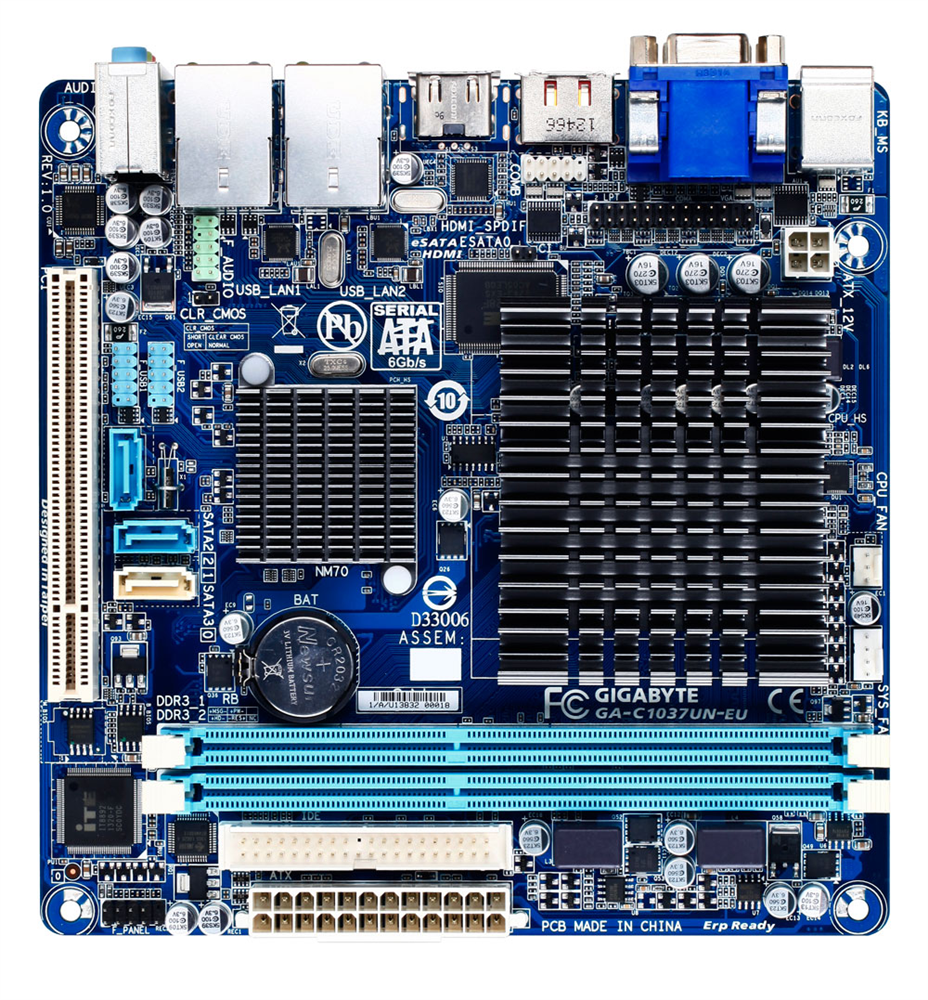
\includegraphics[height=0.45\textheight]{azlin/doc/gac1037.jpg} &
\begin{tabular}{l l}
CPU & Celeron 1037U \\
\ram & 2 $\times$ DDR3, max 16G, 2 канала \\
чипсет & Intel NM70 \\
сеть & 2 $\times$ Realtek® GbE 1Gb (rtl8111) \\
HDD & 2 $\times$ SATA2 (3Gb/s), 1 $\times$ SATA3 (6Gb/s), 1 $\times$ eSATA\\
USB & 6 $\times$ USB3.0 \\
видео & IntelGMA, выходы на VGA D-Sub и HDMI 1.4\\
аудио & Realtek ALC887 (HDA) \\
PCI & $\times$1 \\
&\\
\end{tabular}
\\
\end{tabular}

В качестве варианта 64-битной платформы взята портативная материнка для
неттопов: Gigabyte GA-C1037UN-EU. На ней возможны два варианта сборки:

\begin{enumerate}
  \item \emph{x86\_64/x64}: нативный \verb|CPU=Celeron1037u|
  \item \emph{i686/x32}: режим соместимости со старыми процессорами
  \verb|CPU=i686|
\end{enumerate}

\url{http://www.ixbt.com/news/hard/index.shtml?17/33/31}

\clearpage
На текущий момент эта материнка\ --- оптимальный вариант для офисного, рабочего
неигрового компьютера, или базы для изготовления мобильной рабочей станции в
миникейсе: комплект из GA-C1037UN-EU и блока питания стоит порядка 5 тыс.руб,
при этом возможна установка до 2$\times$8G \ram, что пока недоступно на дешевых
ноутбуках. \emph{Но\ --- \textsc{отвратительный} радиатор на мосте NM70, нагрев
до $70^{o}C$, в обязательном порядке делать сквозную продувку корпуса \textbf{до
включения материнки}.}

\begin{tabular}{l l}
материнская плата& GA-C1037UN-EU rev.2 \\
CPU& Celeron 1037U (впаян) \\
охлаждение& \emph{отвратительное, обязательны кулера на все чипы и сквозная
продувка корпуса},
\\
\ram& 1$\times$8G DDR3 (в планах 2$\times$8G) \\
HDD & \emph{нет}, используется флешка 8G USB3 Transcend JF750 (возможно SATA
SSD) \\
TFT & китайский 3.5'' автомониторчик + конвертер HDMI2RCA на случай\\&
посмотреть видеовывод, обычно везде где я использую эту поделку,\\& есть VGA
монитор или хотя бы большой телевизор\\
электропитание& БП Hipro HPE-350W + автоинвертор\\& батарея не требуется, под
боком всегда есть 220 или 12\,В\\
& по необходимости в транспорт грузится пара заряженных автоаккумуляторов\\
\end{tabular}
\bigskip

\lstx{hw/gac1037.mk}{}{../azlin/hw/gac1037.mk}{mk}\index{azLinux!железо!Gigabyte GA-C1037UN-EU}

\subsection{ARM}

\subsubsection{qemuARM: эмулятор QEMU}
\lstx{hw/qemuARM.mk}{}{../azlin/hw/qemuARM.mk}{mk}\index{azLinux!железо!QEMU}
\subsubsection{cubie1: Cubie Board v.1}
\subsubsection{rpi: Raspberry Pi model B}
\subsection{MIPS}
\subsubsection{qemuMIPS: эмулятор QEMU}
\lstx{hw/qemuMIPS.mk}{}{../azlin/hw/qemuMIPS.mk}{mk}\index{azLinux!железо!QEMU}
\subsubsection{mr3020: роутер MR3020}
\href{http://wiki.openwrt.org/ru/toh/tp-link/tl-mr3020}{mr3020}
\subsubsection{vocore: VoCore} \index{azLinux!железо!VoCore}
\href{http://vocore.io/}{vocore}
\subsubsection{bswift: BlackSwift} \index{azLinux!железо!BlackSwift}
\href{http://habrahabr.ru/post/242731/}{bswift}

\section{CPU: Конфигурации процессоров}

Настройки на процессор задаются в файле \file{cpu/\$\{CPU\}.mk}.

\begin{tabular}{p{0.15\textwidth} p{0.8\textwidth}}
\file{ARCH} & архитектура целевой системы, используется при конфигурировании
ядра \\
\file{TARGET} & \term{триплет целевой системы}, параметр задает тип целевой
системы при сборке кросс-компилятора и используется во всех скриптах
\prog{configure}\ при сборке остальных пакетов \\
\file{CFG\_CPU} & параметры при сборке кросс-компилятора \\
\file{CPU\_FLAGS} & параметры \prog{gcc}\ для оптимизации кода \\
\end{tabular}

\subsection{i386}

\lstx{cpu/i486sx.mk}{}{azlin/cpu/i486sx.mk}{mk}
\index{azLinux!железо!i486sx}

\lstx{cpu/CeleronM.mk}{}{azlin/cpu/CeleronM.mk}{mk}
\index{azLinux!железо!CeleronM}

\lstx{cpu/Celeron1037U.mk}{}{azlin/cpu/Celeron1037U.mk}{mk}
\index{azLinux!железо!Celeron1037U}

\subsection{ARM}
\subsection{MIPS}

\lstx{cpu/AR7240.mk}{}{../azlin/cpu/AR7240.mk}{mk}\index{azLinux!железо!AR7240}

\lstx{cpu/RT5350.mk}{}{../azlin/cpu/RT5350.mk}{mk}\index{azLinux!железо!RT5350}


\section{Пакеты}\label{azpacks}

\subsection{\prog{dirs}: создание дерева каталогов} \label{azdirs}

\subsection{\prog{gz}: закачка архивов исходников} \label{azgz}

\subsection{\prog{tc}: сборка кросс-компилятора} \label{aztc}

\subsubsection{\prog{binutils}: ассемблер, линкер и утилиты} \label{azbinutils}

\subsubsection{\prog{cclibs}: библиотеки для сборки \prog{gcc}} \label{azcclibs}

\prog{gmp} \prog{mpfr} \prog{mpc}

\subsubsection{\prog{gcc0}: сборка минимального кросс-компилятора Си}
\label{azgcc0}

\subsubsection{\prog{gcc}: сборка кросс-компилятора Си/\cpp} \label{az}

Пакет собирается \emph{после сборки \prog{core}}. 

\subsection{\prog{core}: сборка основной системы} \label{azcore}

\subsubsection{\prog{kernel}: ядро \linux} \label{azkernel}

\subsubsection{\prog{libc}: библиотека \prog{uClibc}} \label{azlibc}

\subsubsection{\prog{bb}: набор утилит \prog{busybox}} \label{azbb}

\subsubsection{\prog{gcc}: пересборка полного \prog{gcc}} \label{azgcc}

\subsection{\prog{libs}: сборка библиотек \file{\$\{LIBS\}}} \label{azlibs}

\subsection{\prog{apps}: сборка прикладных пакетов \file{\$\{APPS\}}}
\label{azapps}

\subsection{\prog{user}: сборка пользовательского кода} \label{azuser}

\subsection{\prog{root}: формирование корневой файловой системы} \label{azroot}
\subsection{\prog{boot}: сборка загрузчика} \label{azboot}

\section{\prog{emu}: запуск собранной системы в эмуляторе} \label{azemu}

\section{Сетевая загрузка \file{netboot}} \label{aznetboot}

\section{Прошивка на устройство} \label{azfirmware}
